\subsection{Motivation}

\begin{frame}
  \frametitle{Reactor systems potentially meeting the Generation IV goals}
               \begin{figure}[t]
                \vspace*{-0.1in}
                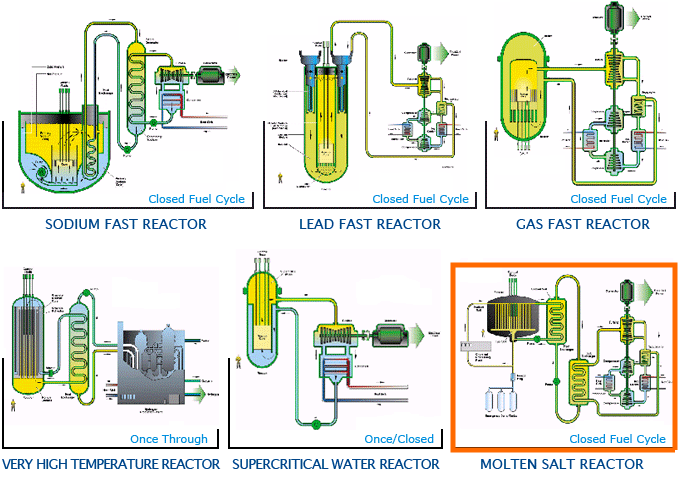
\includegraphics[height=0.65\textwidth]{./images/6_types.png}
                 \caption{Potential Generation IV reactors \cite{ABRAM2008}.}
               \end{figure}
              
\end{frame}

\begin{frame}
  \frametitle{Why Molten Salt Reactors?}
                  \vspace*{-0.1in}
              \begin{block}{Main advantages of liquid-fueled \glspl{MSR}\cite{elsheikh_safety_2013}}
               \begin{enumerate}
                \item High average temperature of coolant (600-750$^{\circ}$C) $\Rightarrow$ high thermal efficiency.
                \item May operate with epithermal or fast neutron spectrums.
                \item Various fuels can be used ($^{235}$U, $^{233}$U, Thorium, U/Pu).
                \item Inherent safety advantages: liquid fuel has strong negative temperature feedback and drains into tanks in emergency.
                \item Large fuel utilization $\Rightarrow$ less nuclear waste generated.
                \item Online reprocessing and refueling.
               \end{enumerate}
               \end{block}
                  \vspace*{-0.1in}               
               \begin{block}{Main advantages of \gls{MSBR}\cite{robertson_conceptual_1971}}
               \begin{enumerate}
                \item Breed fissile $^{233}$U from $^{232}$Th (breeding ratio 1.06).
                \item $^{233}$U, $^{235}$U, or $^{239}$Pu could be used for the initial fissile loading.
                \item Thorium cycle produces a reduced quantity of Pu and minor actinides.
                \item Could operate as a converter reactor for \glspl{LWR} spent fuel transmutation.
               \end{enumerate}
               \end{block}

\end{frame}

\begin{frame}
  \frametitle{Molten Salt Reactor Experiment vs Molten Salt Breeder Reactor}
  \begin{columns}
    \column[t]{5.6cm}
               \begin{figure}[t]
                \vspace*{-0.3in}
                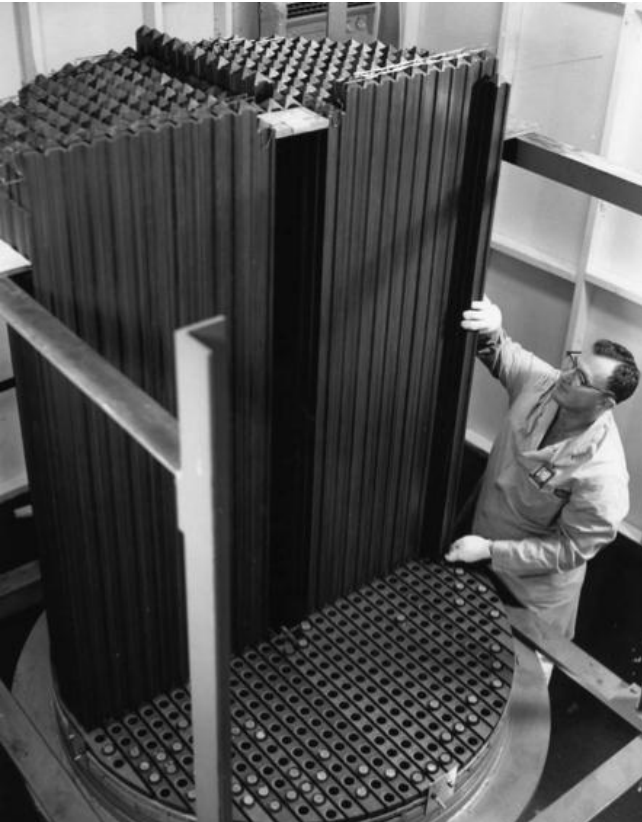
\includegraphics[height=0.7\textwidth]{./images/msre_view.png}
                \vspace*{-0.2in}
      \end{figure}
     \begin{block}{\gls{MSRE}}
       \begin{enumerate}
              \item Maximum power 8 MW$_{th}$
               \item Fuel salt
                \begin{itemize}
                   \item $^7$LiF-BeF$_2$-ZrF$_4$-UF$_4$
                   \item $^7$LiF-BeF$_2$-ZrF$_4$-UF$_4$-PuF$_3$
                \end{itemize}  
              \item First use of $^{233}$U and mixed U/Pu
              \item Single region core
              \item Operated: 1965-1969 at ORNL
              \end{enumerate}
     \end{block}
     \column[t]{5.6cm}
           \begin{figure}[t]
                \vspace*{-0.3in}
                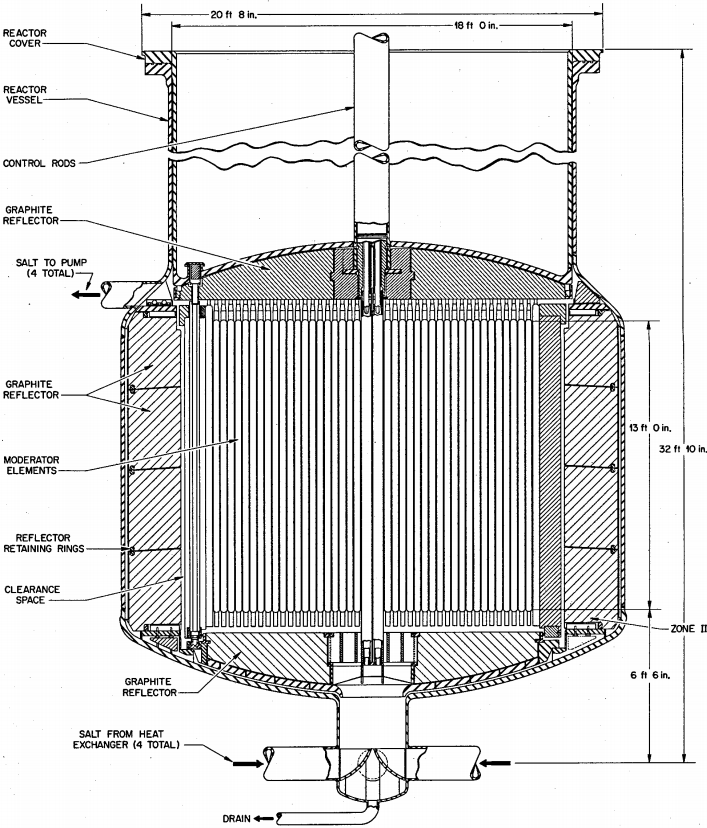
\includegraphics[height=0.7\textwidth]{./images/msbr_plain.png}
                \vspace*{-0.2in}
      \end{figure}
   \begin{block}{\glsfirst{MSBR} \cite{robertson_conceptual_1971}}
       \begin{enumerate}
       \item Maximum power 2.25GW$_{th}$, 1GW$_e$
       \item Fuel salt
         \begin{itemize}
         \item $^7$LiF-BeF$_2$-ThF$_4$-$^{233}$UF$_4$
         \item $^7$LiF-BeF$_2$-ThF$_4$-$^{233}$UF$_4$-$^{239}$PuF$_3$
         \end{itemize}  
       \item Breeding ratio 1.06
       \item Single fluid/two-region core design
       \item Chemical salt processing plant
      \end{enumerate}
     \end{block}
  \end{columns}
              
 \end{frame}

\subsection{Objectives}
\begin{frame}
  \frametitle{Research objectives}
                  \vspace*{-0.1in}
              \begin{block}{Goals of current study}
               \begin{enumerate}
                \item Develop simplified single-cell \gls{MSBR} model using the continuous-energy SERPENT 2 Monte Carlo reactor
					physics software \cite{leppanen_serpent_2012}.
                \item Using the built-in SERPENT 2 depletion  capabilities simulate online reprocessing and refueling regime.
                \item Find the equilibrium core composition for the \gls{MSBR}.
               \end{enumerate}
               \end{block}
               
               \begin{block}{What is next?}
               \begin{enumerate}
                \item Depletion simulation using a full-core, 3-D, high-fidelity \gls{MSBR} model.
                \item Additional SERPENT 2 flow control system will be developed to adjusting material flows.
                \item Optimization of reprocessing parameters and the reactor design.
                \item Determine and compare major safety characteristics for initial and equilibrium fuel composition.
               \end{enumerate}
               \end{block}

\end{frame}

